% LaTeX Template for short student reports.
% Citations should be in bibtex format and go in references.bib
\documentclass[a4paper, 11pt]{article}
\usepackage[top=3cm, bottom=3cm, left=2cm, right=2cm]{geometry} 
\geometry{a4paper} 
\usepackage[utf8]{inputenc}
\usepackage[vietnamese]{babel}
\usepackage{xcolor}
\usepackage{sectsty}
\usepackage{textcomp}
\usepackage{graphicx} 
\usepackage{amsmath,amssymb}
\usepackage{algorithm,algcompatible}
\usepackage{caption}
\usepackage{subcaption}
\usepackage{bm}
\usepackage{tikz}
\usepackage{enumitem}
\setlist[itemize]{leftmargin=*}
\usepackage[pdftex,bookmarks,colorlinks,breaklinks]{hyperref}  
%\hypersetup{linkcolor=black,citecolor=black,filecolor=black,urlcolor=black} % black links, for printed output
\usepackage{memhfixc}
\usepackage{wrapfig}
\usepackage{pdfsync}  
\usepackage{fancyhdr}
\usepackage{pifont}
\usepackage{listings}
\usepackage{lstfiracode}
\lstset{style=FiraCodeStyle,basicstyle=\ttfamily,columns=fullflexible,breaklines=true}
\makeatletter
\def\lst@visiblespace{ }
\makeatother
\usepackage[export]{adjustbox}

\pagestyle{fancy}
\sloppy

\graphicspath{ {images/} }
\setlength{\headheight}{16.50983pt}
\setlength{\parindent}{0pt}

\newenvironment{vnalgorithm}[1][]
  {\begin{algorithm}[#1]
     \selectlanguage{vietnamese}%
     \floatname{algorithm}{Thuật toán}%
     \algnewcommand\INPUT{\item[\textbf{Đầu vào:}]}%
     \algnewcommand\OUTPUT{\item[\textbf{Đầu ra:}]}%
     \algnewcommand\BEGIN{\item[\textbf{begin}]} %
     \algnewcommand\DO{\textbf{ do}} %
     \algnewcommand\RETURN{\State\textbf{return }}%
     \algnewcommand\BREAK{\State\textbf{break}}%
     \algnewcommand\CONTINUE{\State\textbf{continue}}
     \algnewcommand\END{\item[\textbf{end}]}%
     % Set other language requirements
  }
  {\end{algorithm}}


\title{\textbf{Bài tập Thực hành Nhập môn Trí tuệ Nhân tạo tuần 2}}
\author{Nguyễn Lê Ngọc Duy - 20280023 - 20KDL1}
\date{}

\begin{document}
\maketitle
\hypersetup{linkcolor=black}
\tableofcontents

\pagebreak

\section{Bài toán}
\subsection{Mô tả bài toán}
Trong bài báo cáo này, chúng ta sẽ xem xét quy trình tìm ra lời giải cho bài toán sau bằng hai thuật toán BFS và DFS.

Có 3 người truyền giáo và 3 con quỷ ở bờ bên trái của một con sông, cùng với một con thuyền có thể chở được 1 hoặc 2 người. Nếu số quỷ nhiều hơn số người truyền giáo trong một bờ thì số quỷ đó sẽ ăn thịt số người truyền giáo. Tìm cách để đưa tất cả người truyền giáo qua bờ bên phải của sông mà không bị ăn thịt, nghĩa là số người không ít hơn số quỷ ở cùng 1 bờ (bên trái hoặc bên phải).

\subsection{Phân tích không gian trạng thái.}
Gọi $(a, b, k)$ với $0 \leq a, b \leq 3$; trong đó:
\begin{itemize}
    \item $a$ là số người
    \item $b$ là số quỷ ở bờ bên trái
    \item $k = 1$ nếu thuyền ở bên trái, ngược lại $k = 0$.
\end{itemize}
Khi đó, không gian trạng thái của bài toán đuọc xác định như sau:
\begin{itemize}
    \item Trạng thái ban đầu: $(3, 3, 1)$
    \item Thuyền chở qua sông 1 người, hoặc 1 con quỷ, hoặc 1 người và 1 con quỷ, hoặc 2 người, hoặc 2 con quỷ. Như vậy nếu gọi $(x, y)$ lần lượt là số người và số quỷ di chuyển từ bờ bên trái qua bờ bên phải hay ngược lại thì ta có các phép toán chuyển từ trạng thái này sang trạng thái khác là
    \begin{itemize}
        \item $(1, 0)$.
        \item $(0, 1)$.
        \item $(1, 1)$.
        \item $(2, 0)$.
        \item $(0, 2)$.
    \end{itemize}
    \item Trạng thái kết thúc là $(0, 0, 0)$.
\end{itemize}

\clearpage

\section{Tìm hiểu thuật toán.}
\subsection{Thuật toán Breadth First Search - BFS.}
Thuật toán BFS là thuật toán mà trậng thái gốc được duyệt trước, sau đó đến các bước tiếp theo và cuối cùng đến trạng thái gốc. Tổng quát, tất cả các node ở cùng một mức sẽ được khám phá hết, sau đó đến mức tiếp theo.\\ Ta có thể dùng một hàng đợi để lưu trữ các node cần khám phá. Các node mới nhất sẽ được thêm vào cuối hàng đợi, và các node cũ sẽ được loại bỏ khỏi đầu hàng đợi.\\ Dưới đây chính là mã giả cho thuật toán BFS:\\
\begin{vnalgorithm}
    \caption{Thuật toán Breadth First Search - BFS}
    \begin{algorithmic}[1]
        \INPUT{Bài toán}
        \OUTPUT{Lời giải hoặc thông báo: không tồn tại lời giải.}
        \BEGIN
            \STATE{$node \leftarrow$ một node với STATE $=problem.$INITIAL-STATE, PATH-COST $= 0$}
            \IF{$problem.$GOAL-TEST($node.$STATE)}
                \RETURN{SOLUTION($node$)}
            \ENDIF
            \STATE{$frontier \leftarrow$ một hàng đợi với $node$ là phần tử duy nhất.}
            \LOOP \DO
                \IF{EMPTY?($frontier$)}
                    \RETURN{FAILURE}
                \ENDIF
                \STATE{$node \leftarrow$ POP($frontier$)}
                \STATE{Thêm $node.$STATE vào $explored$}
                \FOR {\textbf{each} action \textbf{in} $problem$.ACTIONS($node.$STATE)}
                    \STATE $child \leftarrow$ CHILD-NODE($problem$, $node$, $action$)
                    \IF{$child.$STATE không ở trong $explored$ hay $frontier$}
                        \IF{$problem.$GOAL-TEST($child.$STATE)}
                            \RETURN{SOLUTION($child$)}
                        \ENDIF
                        \STATE{$frontier \leftarrow$ INSERT($child$, $frontier$)}
                    \ENDIF
                \ENDFOR
            \ENDLOOP
        \END
    \end{algorithmic}
\end{vnalgorithm}

\begin{figure}[h]
    \centering
    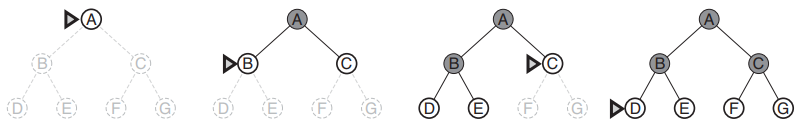
\includegraphics[width=\textwidth,height=\textheight,keepaspectratio]{bfs_demo.png}
    \caption{Minh hoạ thuật toán BFS}
\end{figure}

\subsection{Thuật toán Depth First Search - DFS.}
Khác với thuật toán BFS, thuật toán DFS ưu tiên duyệt tìm node sâu nhất ở trạng thái hiện tại của cây. Quá trình tìm kiếm ngay lập tức tiến đến độ sâu tối đa của cây, khi các node không có node con nào thì quay lại node cha và tìm node con tiếp theo.

Ta sử dụng một ngăn xếp để lưu trữ kết quả tìm kiếm, theo đó, các node vừa được thêm vào ngăn xếp được duyệt trước, và các node cũ sẽ được loại bỏ khỏi ngăn xếp.

\begin{figure}[h]
    \centering
    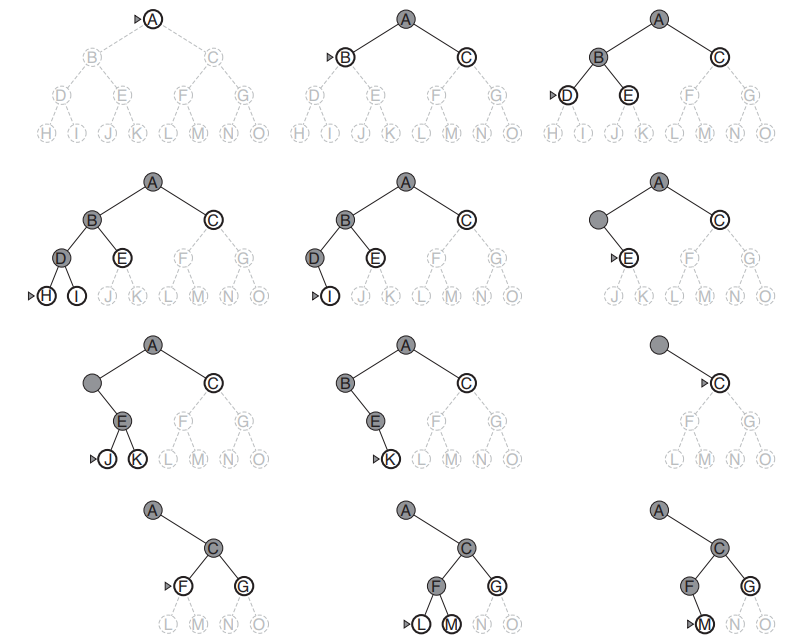
\includegraphics[width=\textwidth,height=\textheight,keepaspectratio]{dfs_demo.png}
    \caption{Minh hoạ thuật toán DFS}
\end{figure}

\subsection{So sánh ban đầu về hai thuật toán.}
Bảng sau so sánh hai thuật toán trên dựa trên 4 tiêu chí: độ hoàn thiện, độ phức tạp thời gian, độ phức tạp không gian và độ tối ưu, trong đó:

\begin{itemize}
    \item $b$: số node con của một node.
    \item $d$: độ sâu của node nông nhất.
    \item $m$: độ sâu tối đa của cây.
    \item ${}^a$: đầy đủ nếu $b$ hữu hạn.
    \item ${}^c$: tối ưu nếu chi phí ở mọi bước là xác định.
\end{itemize}

\begin{center}
    \begin{tabular}{ |c|c|c| }
        \hline
        Thuật toán & BFS & DFS \\
        \hline
        Độ hoàn thiện & $\text{Đầy đủ}^{a}$ & Không đầy đủ \\
        \hline
        Độ phức tạp thời gian & $O(b^d)$ & $O(b^m)$ \\
        \hline
        Độ phức tạp không gian & $O(b^d)$ & $O(bm)$ \\
        \hline
        Độ tối ưu  & ${\text{Tối ưu}}^{c}$ & Không tối ưu \\
        \hline
    \end{tabular}
\end{center}

\section{Cài đặt bằng \lstinline|Python|}
\subsection{Các thư viện hỗ trợ}
\begin{itemize}
    \item\lstinline|graphviz|: Là thư viện mã nguồn mở giúp hỗ trợ cho việc minh hoạ các đồ thị với các tính năng hữu dụng như chỉnh font chữ, màu sắc, nét vẽ,...
    \item\lstinline|pydot|: Đây là thư viện hỗ trợ cùng thư viện \lstinline|graphviz| cho \lstinline|Python|. Thư viện hỗ trợ xuất các đồ thị dưới dạng hình ảnh.
    \item\lstinline|pyparsing|: Đây là thư viện hỗ trợ xuất chuỗi dưới các định dạng đặc biệt do người dùng tự tạo ra.
    \item\lstinline|emoji|: Thư viện tạo ra các emoji, thường được sử dụng trong xử lý ngôn ngữ.
\end{itemize}

\begin{figure}[h]
    \centering
    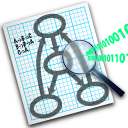
\includegraphics[]{graphviz.png}
    \caption{Thư viện graphviz}
\end{figure}

\subsection{Các file}
\subsubsection{File \lstinline|generate_full_space_tree.py|}
Chức năng chính của file này là tạo ra một cây tìm kiếm và vẽ cây tìm kiếm này ra một file ảnh, bao gồm một số hàm sau:
\begin{itemize}
    \item \lstinline|is_valid_move(number_missionaries, number_cannibals)|: kiểm tra xem một nước đi nào đó có thoả ràng buộc hay không.
    \item \lstinline|draw_edge(number_missionaries, number_cannibals, side, depth_level, node_num)|: vẽ hai trạng thái nào đó và cạnh nối hai trạng thái đó với nhau. Nếu là trạng thái bắt đầu, hàm chỉ vẽ node mà không vẽ cạnh nối.
    \item \lstinline|write_image(file_name="state_space")|: xuất ra file ảnh có dạng \lstinline|{file_name}_{max_depth}.png| (với \lstinline|max_depth| là độ sâu tối đa của cây) đồ thị đã vẽ được.
    \item \lstinline|is_start_state(number_missionaries, number_cannibals, side)|: kiểm tra xem trạng thái nào đó có phải là trạng thái ban đầu không.
    \item \lstinline|is_goal_state(number_missionaries, number_cannibals, side)|: kiểm tra xem trạng thái nào đó có phải là trạng thái kết thúc không.
    \item \lstinline|number_of_cannibals_exceeds(number_missionaries, number_cannibals)|: kiểm tra xem trạng thái nào đó có đạt đến ngưỡng giới hạn không.
    \item \lstinline|generate()|: đây là hàm chính, giúp hình thành lời giải của bài toán. Hàm trả về \lstinline|True| nếu đi đến được độ sâu sâu nhất của cây, ngược lại trả về \lstinline|False|.
\end{itemize}
Ngoài ra, ta tạo thêm tham số dòng lệnh \lstinline|-d| quyết định độ sâu của cây ta muốn tạo (mặc định là 20).

\subsubsection{File \lstinline|solve.py|}
Trong file này, chúng ta viết một lớp \lstinline|Solution| cùng một số các thuộc tính và phương thức để thuận tiện hơn cho việc đi tìm lời giải của bài toán. 

Các thuộc tính của lớp nằm ở trong hàm \lstinline|__init__()| bao gồm:
\begin{itemize}
    \item \lstinline|self.start_state = (3, 3, 1)|: trạng thái ban đầu của bài toán.
    \item \lstinline|self.goal_state = (0, 0, 0)|: trạng thái mục tiêu của bài toán.
    \item \lstinline|self.options = [(1, 0), (0, 1), (1, 1), (0, 2), (2, 0)]|: các toán tử chuyển trạng thái của bài toán.
    \item \lstinline|self.boat_side = ["right", "left"]|: vị trí của con thuyền (bờ phải hoặc bờ trái).
    \item \lstinline|self.graph = pydot.Dot(graph_type='graph', bgcolor="#fff3af", label="fig: Missionaries and Cannibal State Space Tree", fontcolor="red", fontsize="24")|: đồ thị lưu các node trạng thái của bài toán, mặc định ban đầu đồ thị có một node, nền màu da, chữ màu đỏ\dots
    \item \lstinline|self.visited = {}|: một list lưu trữ các trạng thái đã duyệt.
    \item \lstinline|self.solved = False|: cho biết bài toán có giải được hay không.
\end{itemize}

Các phương thức trong lớp này bao gồm:
\begin{itemize}
    \item \lstinline|is_valid_move(self, number_missionaries, number_cannibals)|: kiểm tra xem một nước đi nào đó có thoả ràng buộc hay không.
    \item \lstinline|is_start_state(self, number_missionaries, number_cannibals, side)|: kiểm tra xem trạng thái nào đó có phải là trạng thái ban đầu không.
    \item \lstinline|is_goal_state(self, number_missionaries, number_cannibals, side)|: kiểm tra xem trạng thái nào đó có phải là trạng thái kết thúc không.
    \item \lstinline|number_of_cannibals_exceeds(self, number_missionaries, number_cannibals)|: kiểm tra xem trạng thái nào đó có đạt đến ngưỡng giới hạn không.
    \item \lstinline|write_image(self, file_name="state_space.png")|: hàm này dùng để lưu đồ thị ra file ảnh.
    \item \lstinline|draw_edge(self, number_missionaries, number_cannibals, side, depth_level)|: vẽ hai trạng thái nào đó và cạnh nối hai trạng thái đó với nhau. Nếu là trạng thái bắt đầu, hàm chỉ vẽ node mà không vẽ cạnh nối.
    \item \lstinline|draw_legend(self)|: hàm này dùng để ghi chú thích trên đồ thị.
    \item \lstinline|draw(self, *, number_missionaries_left, number_cannibals_left,    number_missionaries_right, number_cannibals_right)|: hàm này dùng để hiển thị trình tự các trạng thái trên console.
    \item \lstinline|bfs(self)|: hàm này dùng để thực hiện thuật toán BFS.
    \item \lstinline|dfs(self, number_missionaries, number_cannibals, side, depth_level)|: hàm này dùng để thực hiện thuật toán DFS. Khác với hàm  \lstinline|bfs(self)|, ta thêm các tham số để có thể gọi đệ quy hàm này nhiều lần.
\end{itemize}

\subsubsection{File \lstinline|main.py|}
Nhiệm vụ chính của file này là tạo ra một đối tượng của lớp \lstinline|Solution| và gọi đến các phương thức của lớp đó để giải bài toán. Trong file này, ta còn có thêm một số tham số dòng lệnh đi kèm:
\begin{itemize}
    \item \lstinline|-m|: phương thức nào được sử dụng (\lstinline|bfs| hoặc \lstinline|dfs|).
    \item \lstinline|-l|: quyết định xem có chú thích cho đồ thị hay không (\lstinline|True| hoặc \lstinline|False|).
\end{itemize}

\section{Kết quả}

\subsection{Khởi tạo cây không gian trạng thái}

Gõ lệnh \lstinline|python generate_full_space_tree.py -d 8| trên terminal, ta thu được kết quả như hình 4:

\begin{figure}[h]
    \centering
    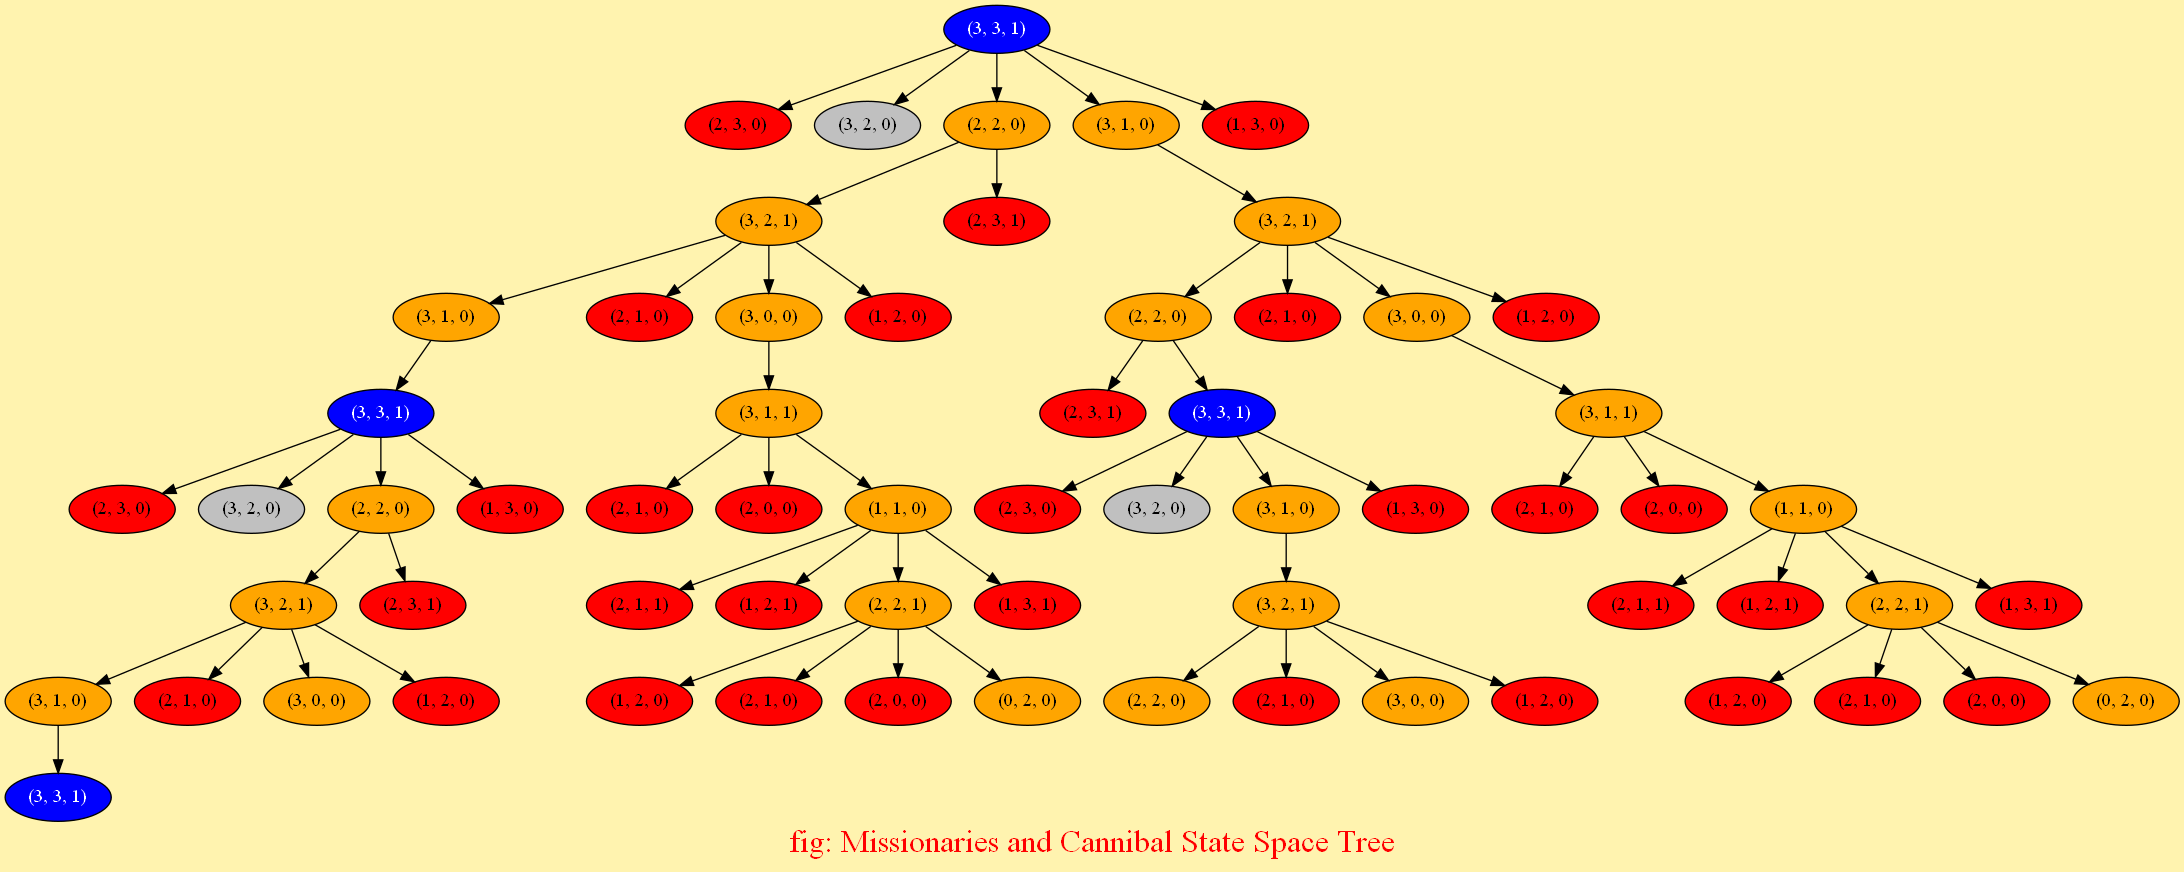
\includegraphics[width=\textwidth,height=\textheight,keepaspectratio]{state_space_8.png}
    \caption{Cây không gian trạng thái cho bài toán với độ sâu tối đa là 8}
\end{figure}

Nếu ta gõ lệnh trên terminal \lstinline|python generate_full_space_tree.py -d 20|, tức là thay đổi độ sâu tối đa của cây tìm kiếm thành 20, ta thu được cây tìm kiếm như hình 5:

\begin{figure}[h]
    \centering
    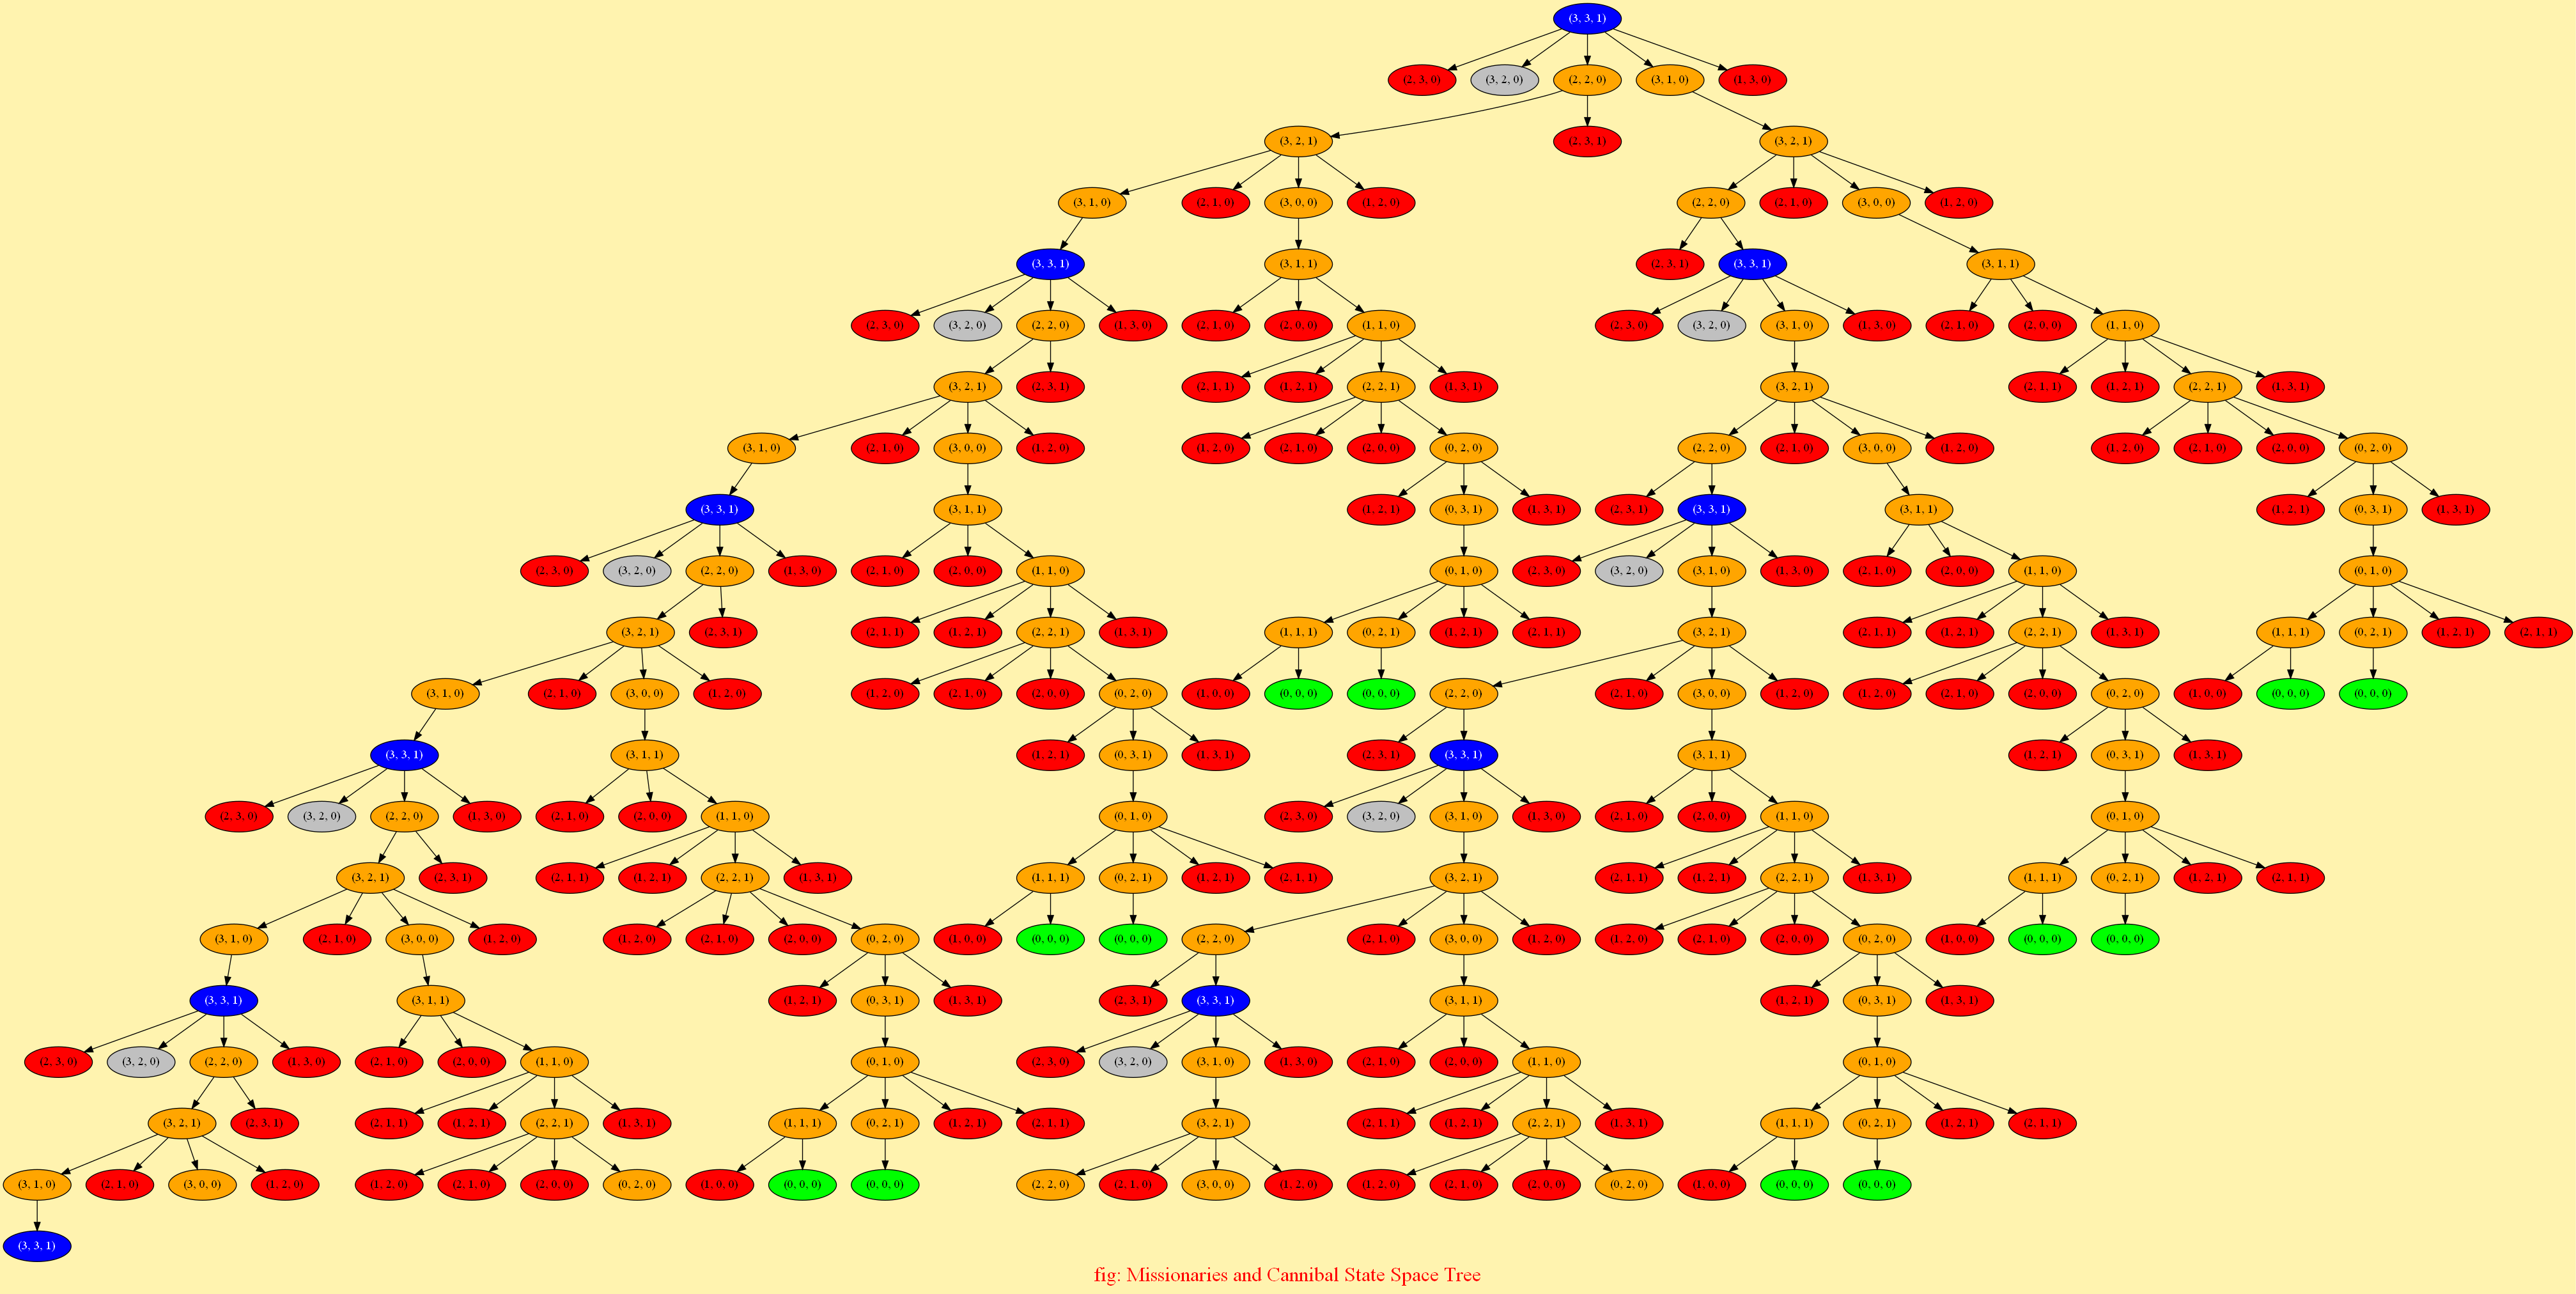
\includegraphics[width=\textwidth,height=\textheight,keepaspectratio]{state_space_20.png}
    \caption{Cây không gian trạng thái cho bài toán với độ sâu tối đa là 20}
\end{figure}

Có thế thấy được rằng khi tăng độ sâu tối đa của cây tìm kiếm lên 20, ta có thể thu được lời giải của bài toán. Ngược lại, nếu độ sâu tối da của cây tìm kiếm là 8, ta không thể tìm được lời giải của bài toán.

\subsection{Giải bài toán với DFS}

Thực thi lệnh \lstinline|python main.py -m dfs|, ta thu được kết quả trên màn hình comsole ở hình 6 và file \lstinline|dfs.png| như hình 8a. Do thuật toán DFS ưu tiên duyệt trạng thái theo chiều sâu, cho nên ta có thể thấy lời giải của bài toán nghiêng hằn về bên tay phải (các node màu vàng).

Để chú thích cây tìm kiếm, ta thực thi lệnh \lstinline|python main.py -m dfs -l True|, ta thu được kết quả trên màn hình comsole ở hình 7 và file \lstinline|dfs_legend.png| như hình 8b.

\begin{figure}[H]
    \centering
    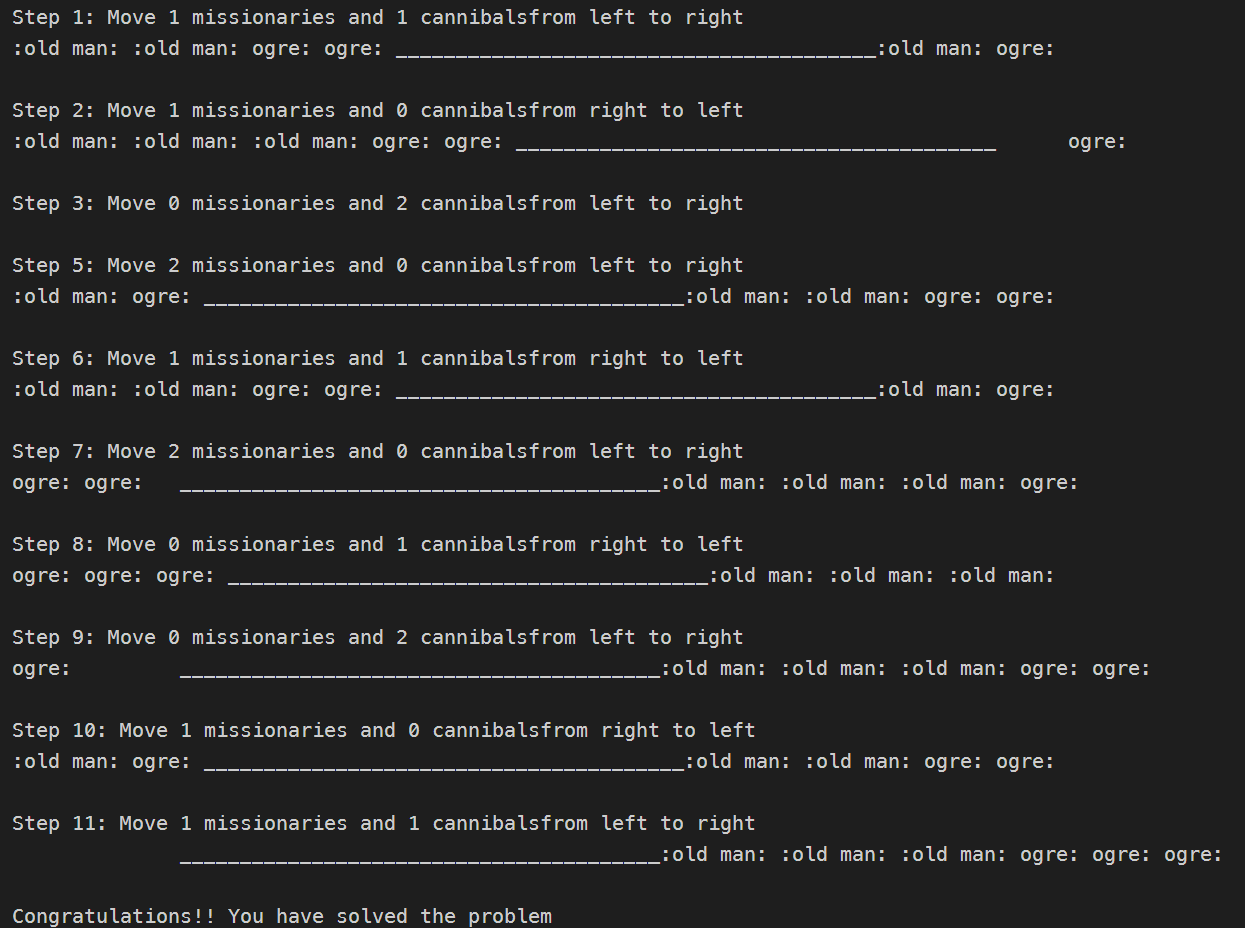
\includegraphics[width=0.8\textwidth,height=0.8\textheight,keepaspectratio]{dfs_console.png}
    \caption{Màn hình console cho thuật toán DFS và không chú thích đồ thị}
\end{figure}

\begin{figure}[H]
    \centering
    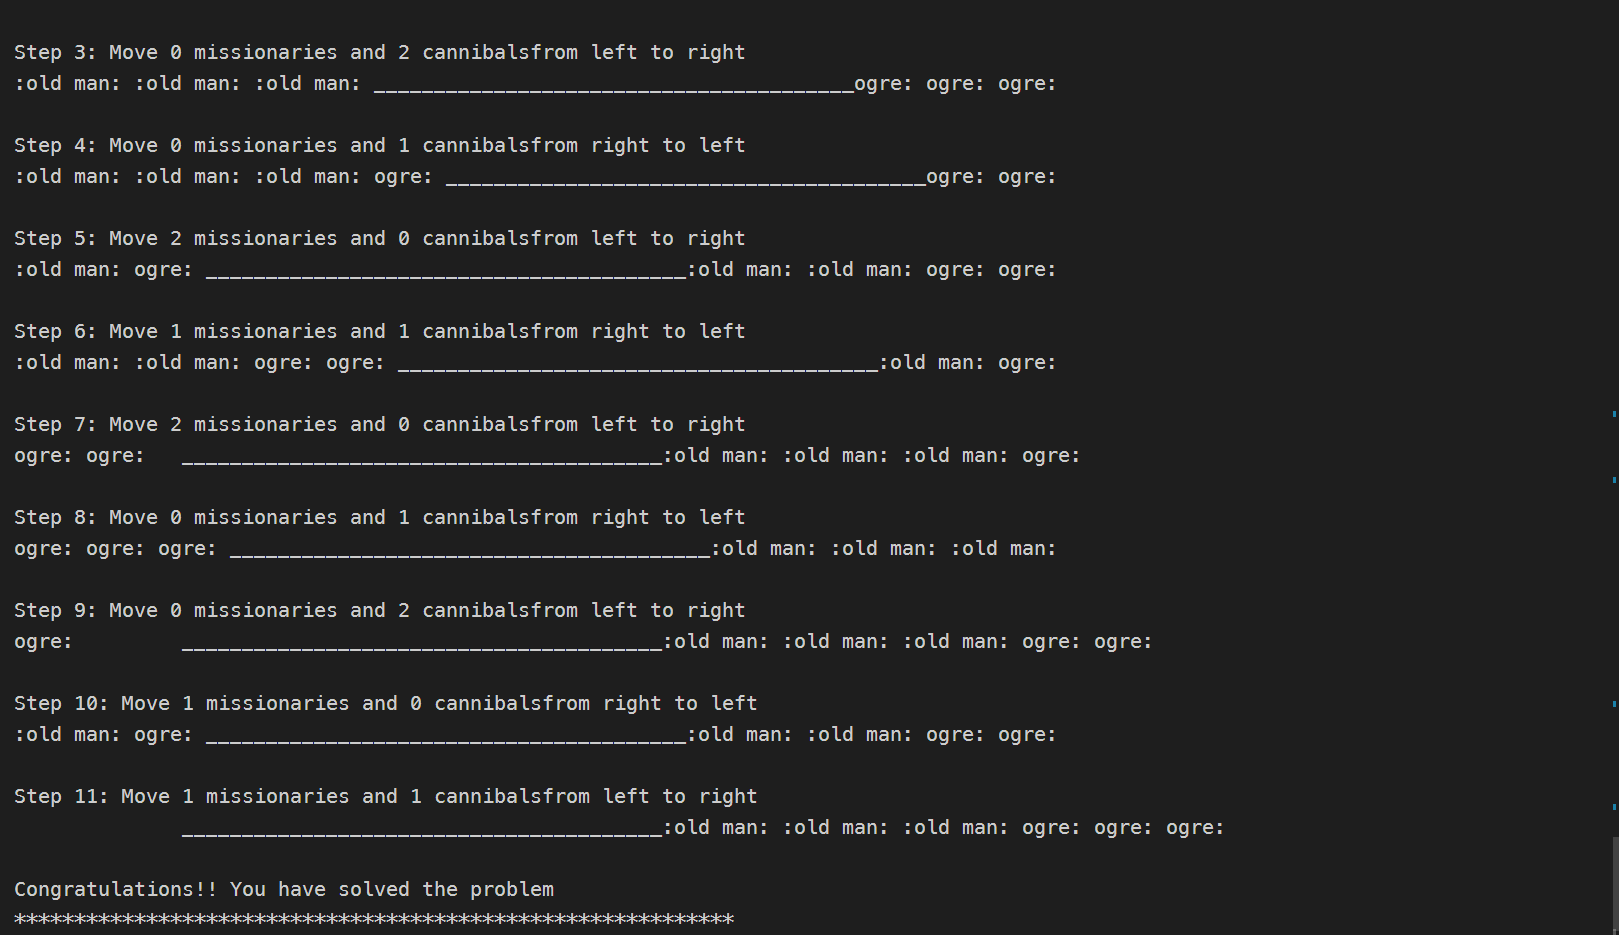
\includegraphics[width=0.8\textwidth,height=0.8\textheight,keepaspectratio]{dfs_console_legend.png}
    \caption{Màn hình console cho thuật toán DFS và có chú thích đồ thị}
\end{figure}

\begin{figure}
    \begin{subfigure}[b]{0.5\textwidth}
        \centering
        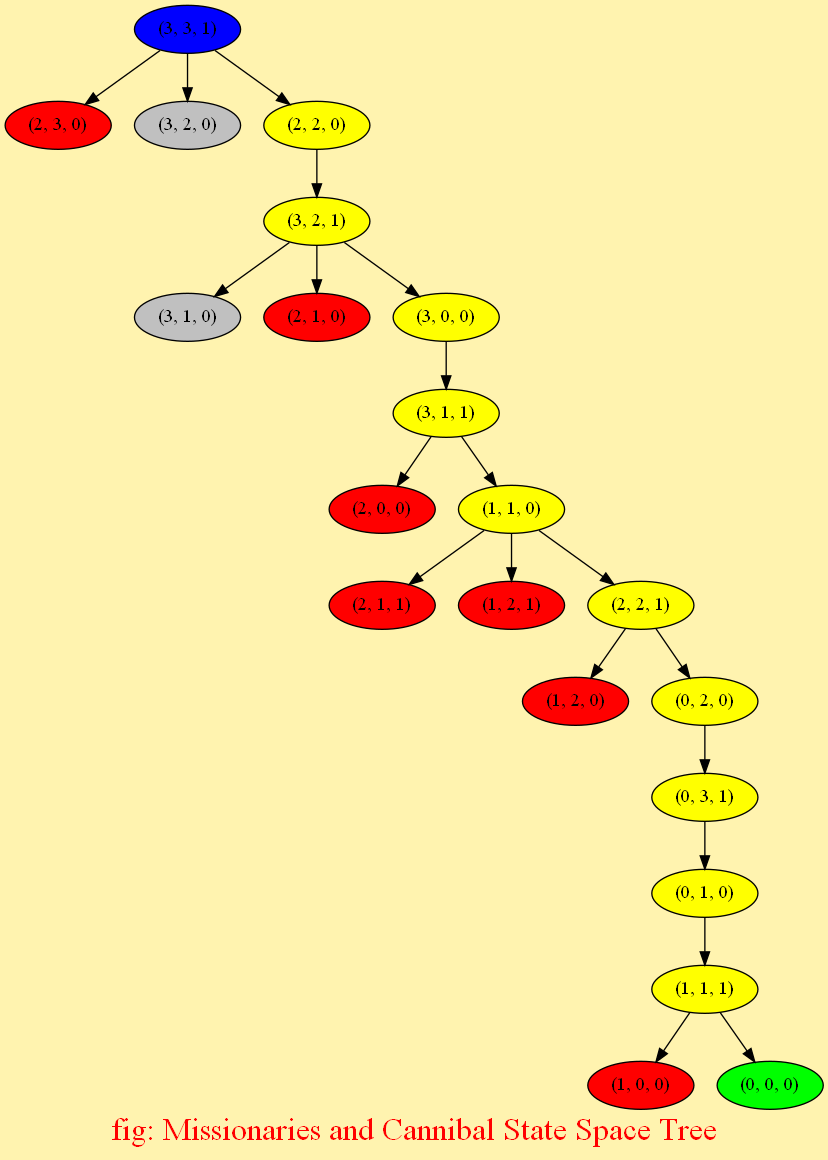
\includegraphics[width=\textwidth]{dfs.png}
        \caption{Không chú thích đồ thị}
    \end{subfigure}
    \hfill
    \begin{subfigure}[b]{0.5\textwidth}
        \centering
        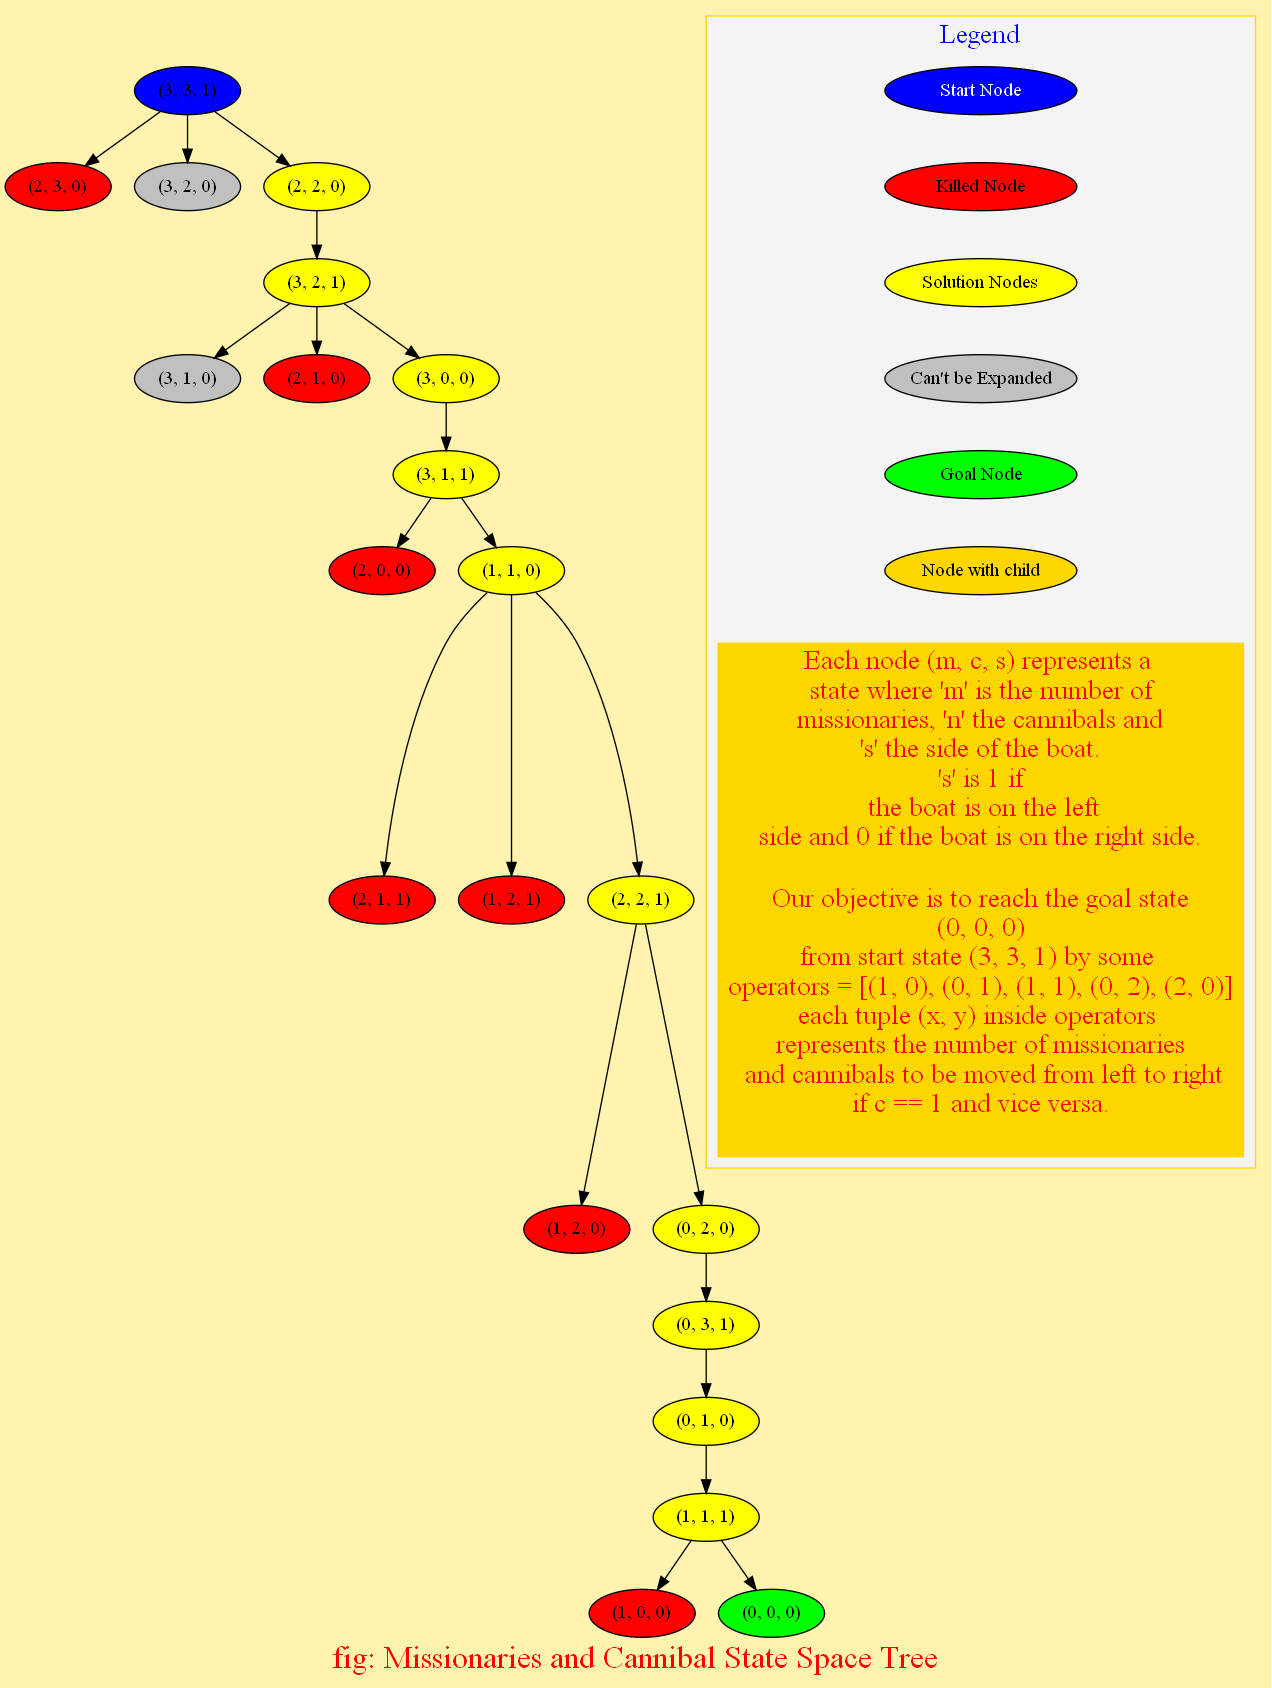
\includegraphics[width=\textwidth]{dfs_legend.png}
        \caption{Có chú thích đồ thị}
    \end{subfigure}
    \caption{Cây tìm kiếm trạng thái bằng thuật toán DFS}
\end{figure}

\subsection{Giải bài toán với BFS}

Thực thi lệnh \lstinline|python main.py -m bfs|, ta thu được kết quả trên màn hình comsole ở hình 9 và file \lstinline|bfs.png| như hình 11a. Do thuật toán BFS ưu tiên duyệt trạng thái theo chiều rộng, cho nên ta có thể thấy các node được mở rộng ra theo nhiều hướng hơn so với thuật toán DFS.

Để chú thích cây tìm kiếm, ta thực thi lệnh \lstinline|python main.py -m dfs -l True|, ta thu được kết quả trên màn hình comsole ở hình 10 và file \lstinline|bfs_legend.png| như hình 11b.

\begin{figure}[H]
    \centering
    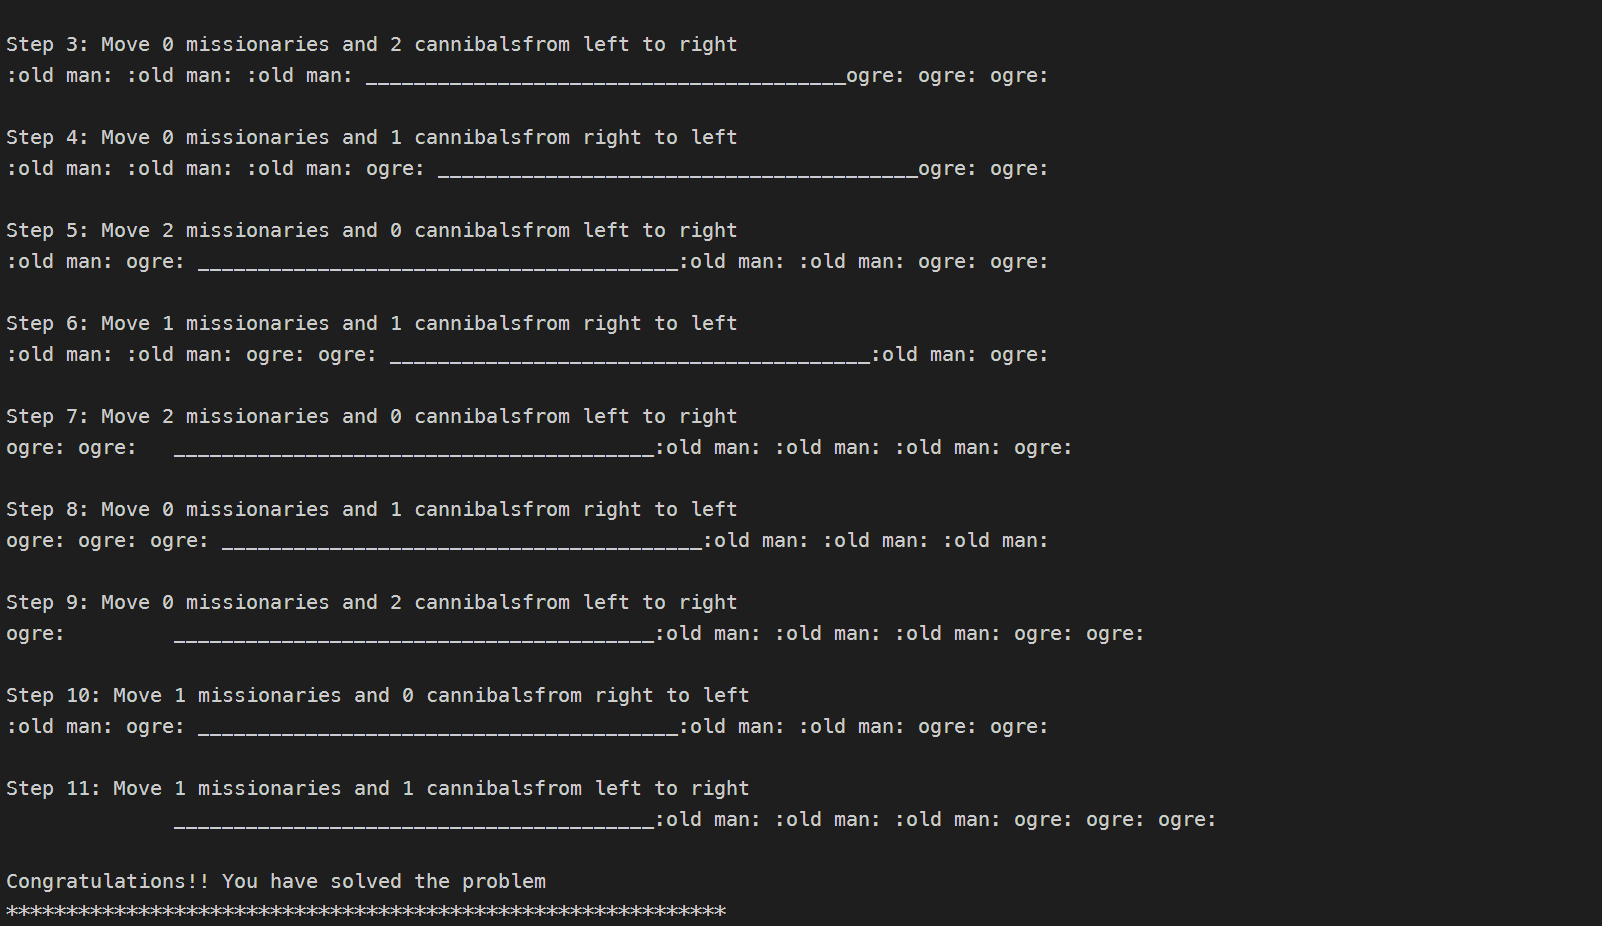
\includegraphics[width=0.8\textwidth,height=0.8\textheight,keepaspectratio]{bfs_console.png}
    \caption{Màn hình console cho thuật toán BFS và không chú thích đồ thị}
\end{figure}

\begin{figure}[H]
    \centering
    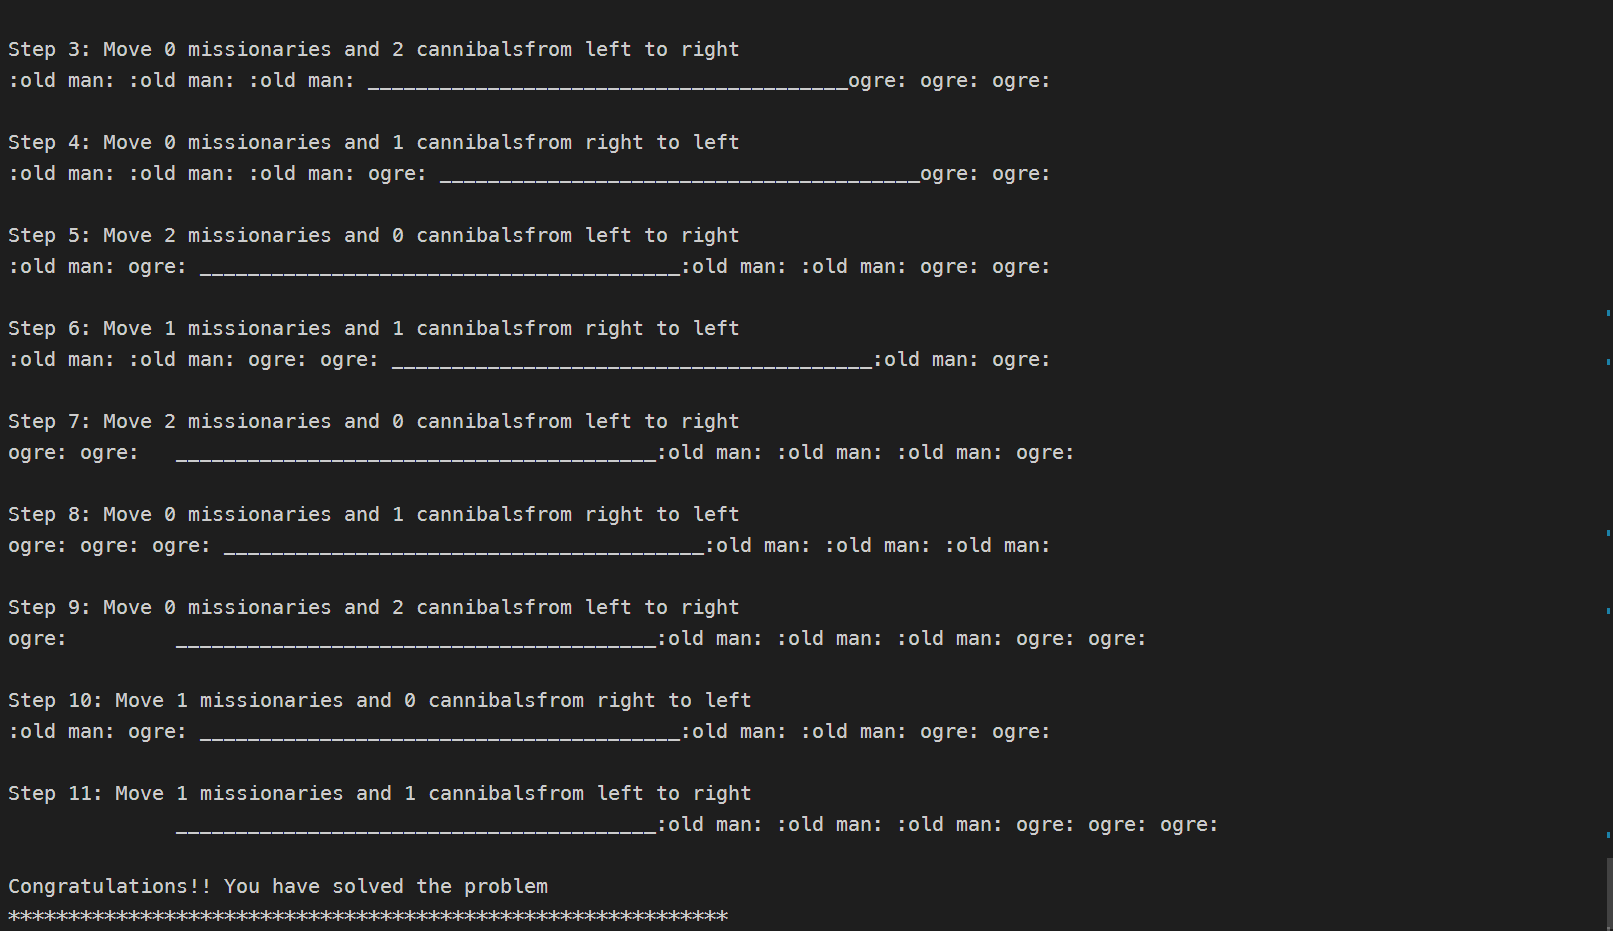
\includegraphics[width=0.8\textwidth,height=0.8\textheight,keepaspectratio]{bfs_console_legend.png}
    \caption{Màn hình console cho thuật toán BFS và có chú thích đồ thị}
\end{figure}

\begin{figure}
    \begin{subfigure}[b]{0.5\textwidth}
        \centering
        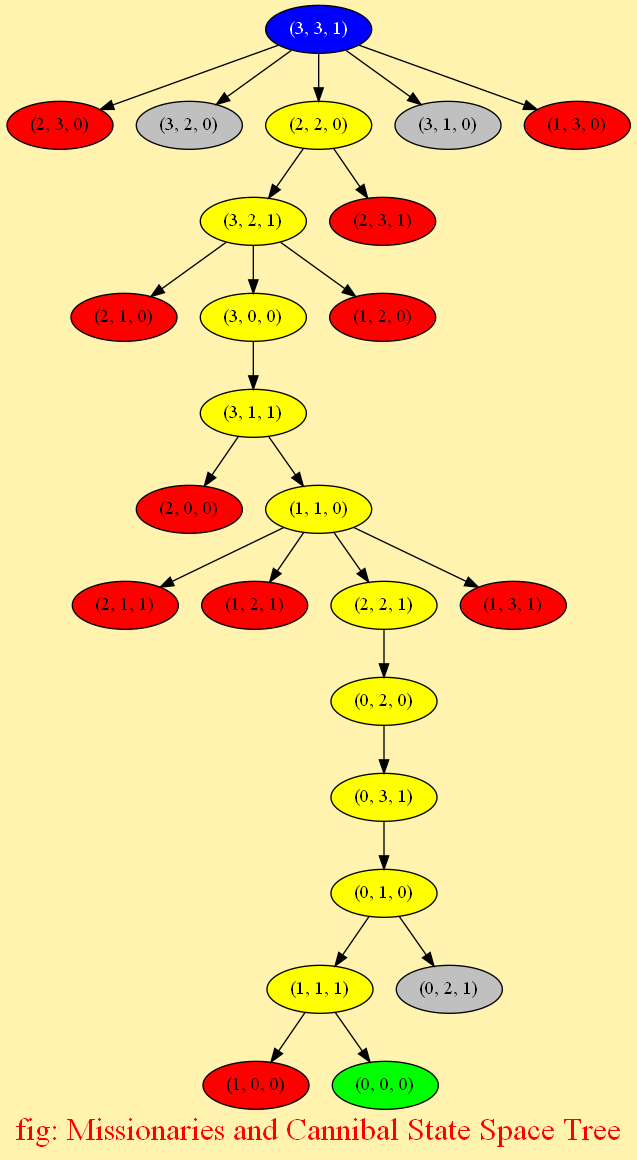
\includegraphics[width=\textwidth]{bfs.png}
        \caption{Không chú thích đồ thị}
    \end{subfigure}
    \hfill
    \begin{subfigure}[b]{0.5\textwidth}
        \centering
        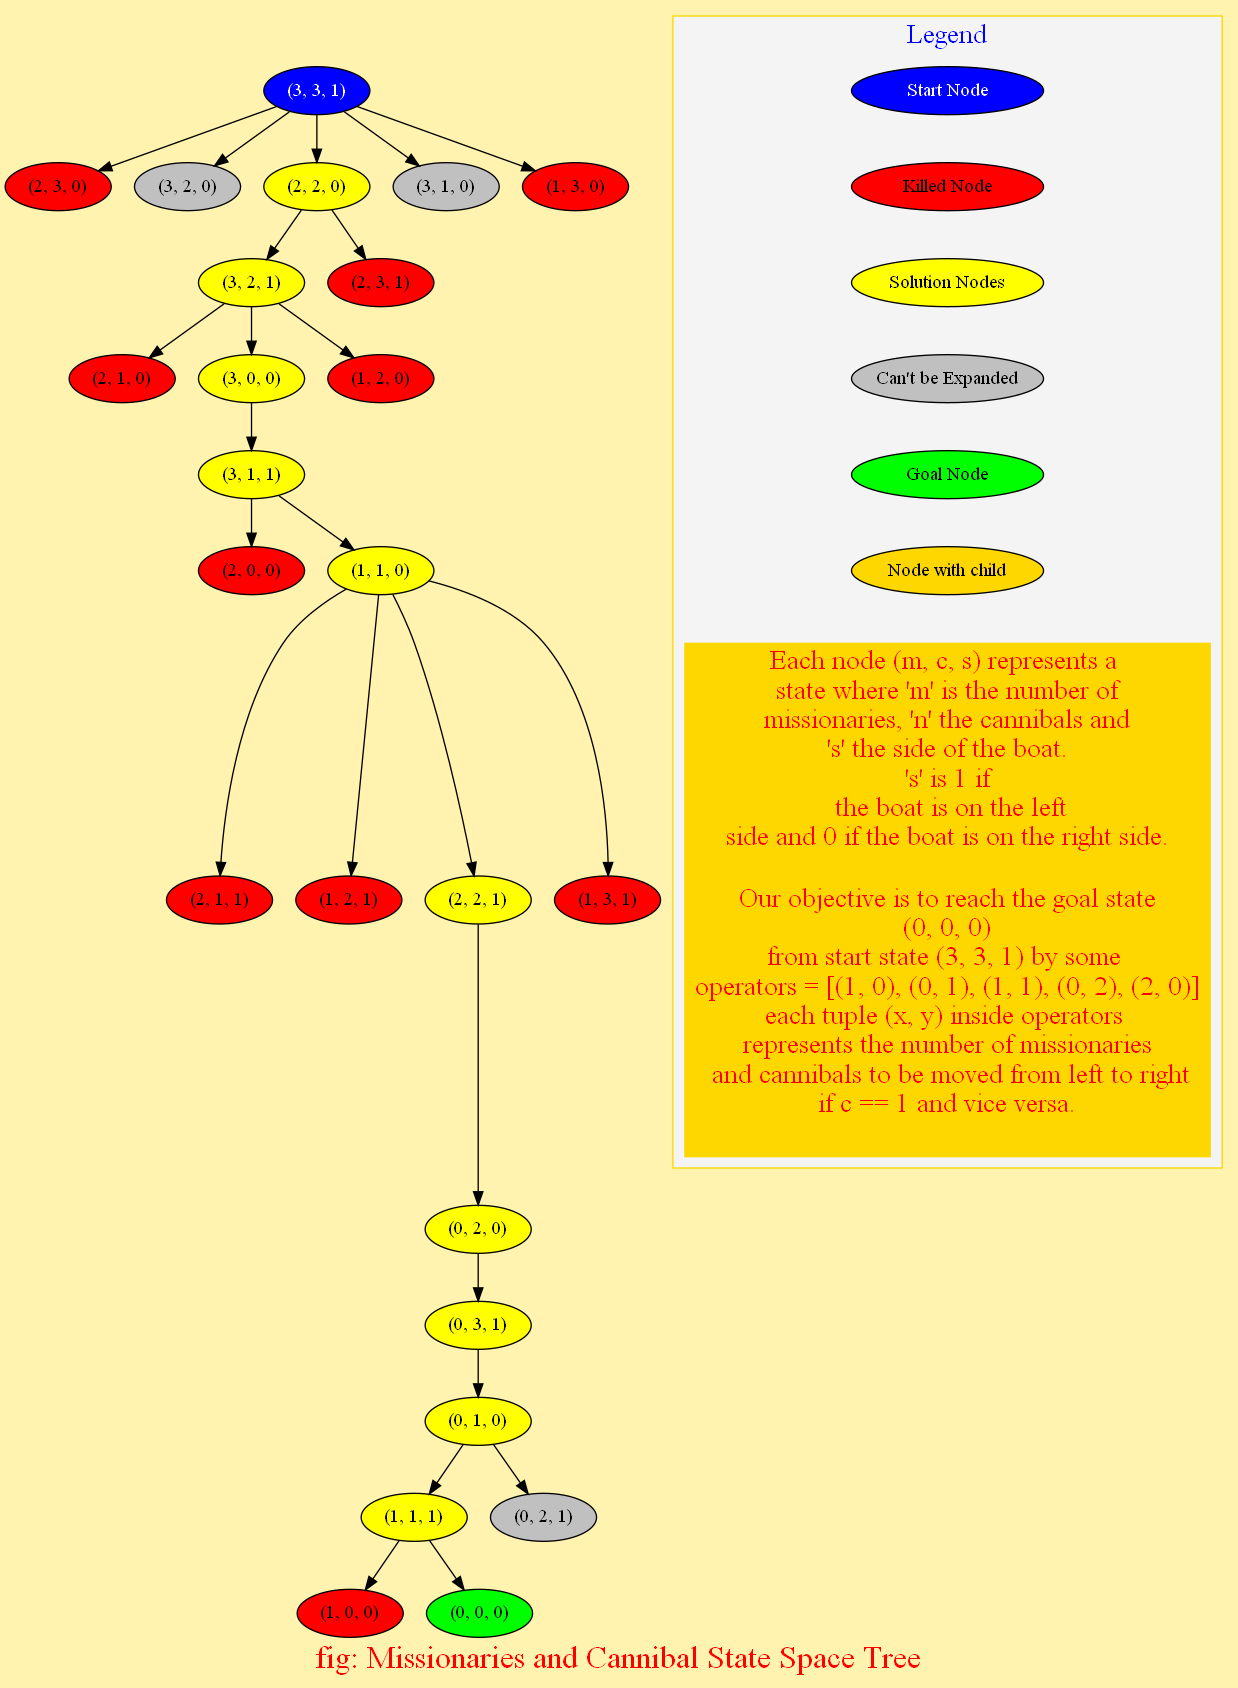
\includegraphics[width=\textwidth]{bfs_legend.png}
        \caption{Có chú thích đồ thị}
    \end{subfigure}
    \caption{Cây tìm kiếm trạng thái bằng thuật toán BFS}
\end{figure}

\clearpage

\subsection{Nhận xét}
Cả hai thuật toán đều tìm được đáp án cho bài toán, nhưng thuật toán DFS tìm được đáp án nhanh hơn so với thuật toán BFS. Điều này có thể giải thích bằng cách nhìn vào cây tìm kiếm của hai thuật toán. Thuật toán DFS tìm kiếm theo chiều sâu, nên nó sẽ mở rộng các node ở mức thấp nhất trước, sau đó mới mở rộng các node ở mức cao hơn. Trong khi đó, thuật toán BFS tìm kiếm theo chiều rộng, nên nó sẽ mở rộng các node ở mức thấp nhất theo thứ tự từ trái sang phải, sau đó mới mở rộng các node ở mức cao hơn. Do đó, thuật toán DFS tìm được đáp án nhanh hơn so với thuật toán BFS.

\section{Tham khảo}
\begin{enumerate}
    \item Thư viện \lstinline|graphviz|: \url{https://www.graphviz.org/}
    \item Thư viện \lstinline|pydot|: \url{https://github.com/pydot/pydot}
    \item Thư viện \lstinline|pyparsing|: \url{https://github.com/pyparsing/pyparsing/}
    \item Thư viện \lstinline|emoji|: \url{https://github.com/carpedm20/emoji/}
    \item Stuart J. Russell, Peter Norvig (2010), Aritificial Intelligence: A Modern Approach, 3rd Edition, Prentice Hall, ISBN-13: 978-0-13-604259-4, ISBN-10: 0-13-604259-7 (\url{https://zoo.cs.yale.edu/classes/cs470/materials/aima2010.pdf})
\end{enumerate}
% \bibliography{references}  % need to put bibtex references in references.bib 
\end{document}